\documentclass[10pt]{beamer}

\usetheme[progressbar=frametitle]{metropolis}
\usepackage{appendixnumberbeamer}

\usepackage{booktabs}
\usepackage[scale=2]{ccicons}

\usepackage{pgfplots}
\usepgfplotslibrary{dateplot}

\usepackage{media9} % Used to include videos

\usepackage{xspace}
\newcommand{\themename}{\textbf{\textsc{metropolis}}\xspace}

\usepackage{array}
\usepackage{longtable}
\usepackage{rotating}
\usepackage{float}
\usepackage{rotfloat}
\usepackage{multirow}
\usepackage{amssymb}
\usepackage{graphicx}
\usepackage{setspace}
\usepackage{nomencl}


%Packages of mindmap

\usepackage[utf8]{inputenc}
%\usepackage{dtklogos}
\usepackage{tikz}
\usetikzlibrary{mindmap,shadows}
% Information boxes
\newcommand*{\info}[4][16.3]{%
  \node [ annotation, #3, scale=0.65, text width = #1em,
          inner sep = 2mm ] at (#2) {%
  \list{$\bullet$}{\topsep=0pt\itemsep=0pt\parsep=0pt
    \parskip=0pt\labelwidth=8pt\leftmargin=8pt
    \itemindent=0pt\labelsep=2pt}%
    #4
  \endlist
  };
}

% Tikz

\definecolor{myblue}{HTML}{020364}
\usetikzlibrary{shapes,arrows,matrix,decorations.pathreplacing,shapes.geometric,positioning}  
% Gantt
\usepackage{pgfgantt}
\usepackage{adjustbox} %Ajustar a la página


\title{Passive dynamic system for energy returning on trans-tibial prosthesis}
\subtitle{Ph.D Thesis Overview}
\date{\today}
\date{}
\author{Nikolay Prieto M.Sc.}
\institute{Dr.Ing. Carlos Julio Cort\'es, Andr\'es Tovar Ph.D. }
\titlegraphic{\hfill
\includegraphics[height=1.5cm]{2.png}}

\begin{document}

\maketitle

\begin{frame}{Table of contents}
  \setbeamertemplate{section in toc}[sections numbered]
  \tableofcontents[hideallsubsections]
\end{frame}

\section{Introduction}

\begin{frame}[fragile]{Introduction}

The purpose of this presentation is to let you know the general research question, the objectives, activities done to date and the tasks in this internship.

\end{frame}

\begin{frame}[fragile]{Introduction}

\begin{figure}[H]
\begin{centering}
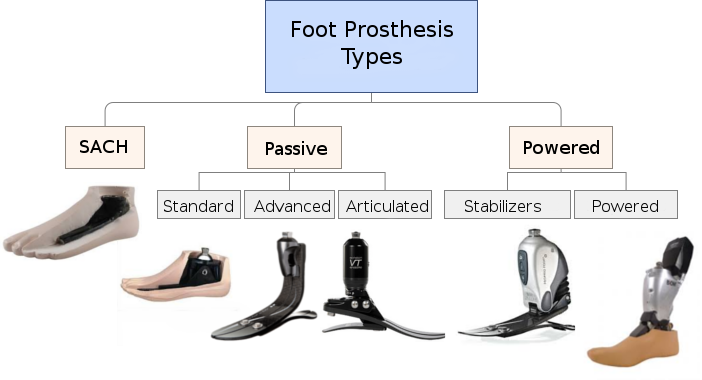
\includegraphics[scale=0.4]{GeneracionesprotesisEng}
\par\end{centering}

\caption{\label{fig:Categorizaci=0000F3n-seg=0000FAn-Cherelle} Generalized categorization of ankle-foot prosthesis according to Cherelle \emph{et al.}\cite{Cherelle2014a} and Versluys \emph{et al.} \cite{Versluys2009}. From left to right: SACH foot, sagital degree of freedom foot, OSSUR$\circledR$ flex foot, Echelon foot$\circledR$, Proprio foot from OSSUR$\circledR$ and BiOM$\circledR$ from iWalk Inc.}
\end{figure}
\end{frame}

\begin{frame}
\begin{figure}[H]
\begin{centering}
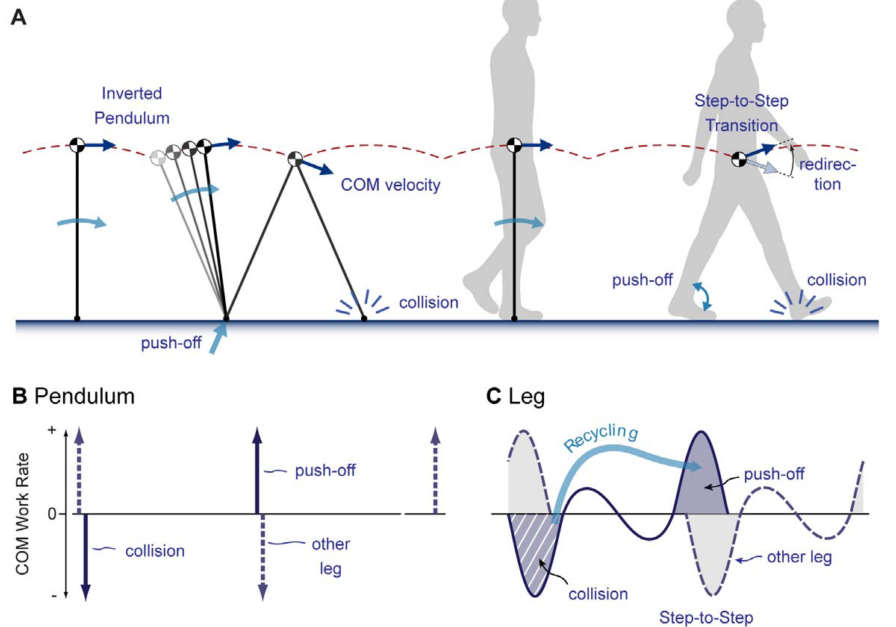
\includegraphics[scale=0.3]{RecycledEng}
\par\end{centering}

\caption{\label{fig:(A)-Representaci=0000F3n-de}{\scriptsize \emph{(A) Synthesizing bipedal walking to an inverted pendulum to support the body COM. The COM velocity is redirected between steps when the other leg contacts the ground with a dissipative collision. (B) The rate of work performed on the COM by ideal pendulum-like legs vs. stride time. Work is theoretically minimized by pushing off impulsively (indicated by arrows) just before the opposite leg’s collision" }Paragraph and figure taken from Collins and Kuo\cite{Collins2010}.}}

\end{figure}
\end{frame}

\begin{frame}[fragile]{Dynamic Joint stiffness}
\begin{figure}[h]
\begin{center}
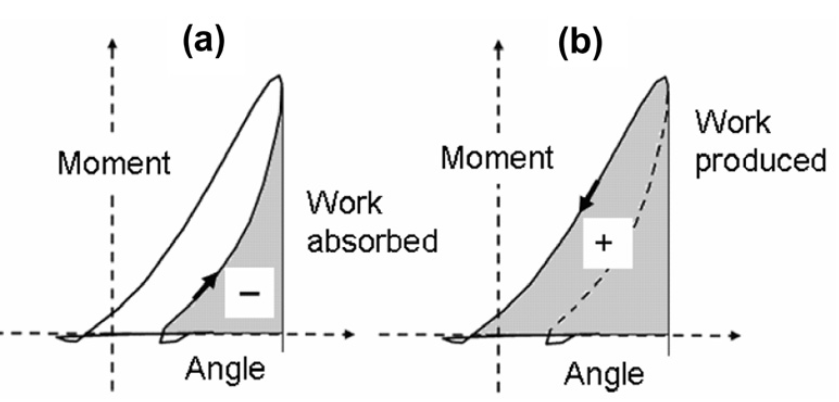
\includegraphics[scale=0.35]{Wproduced.png}
\caption{Representation of Work Produced, Net work and Work Absorbed Section with particular reference to the work absorbed (left panel) and work produced (right panel) in ankle DJS\cite{Crenna2011}.}
\end{center}
\end{figure}
\end{frame}

\begin{frame}[fragile]{Dynamic Joint stiffness}
\begin{figure}[h]
\begin{center}
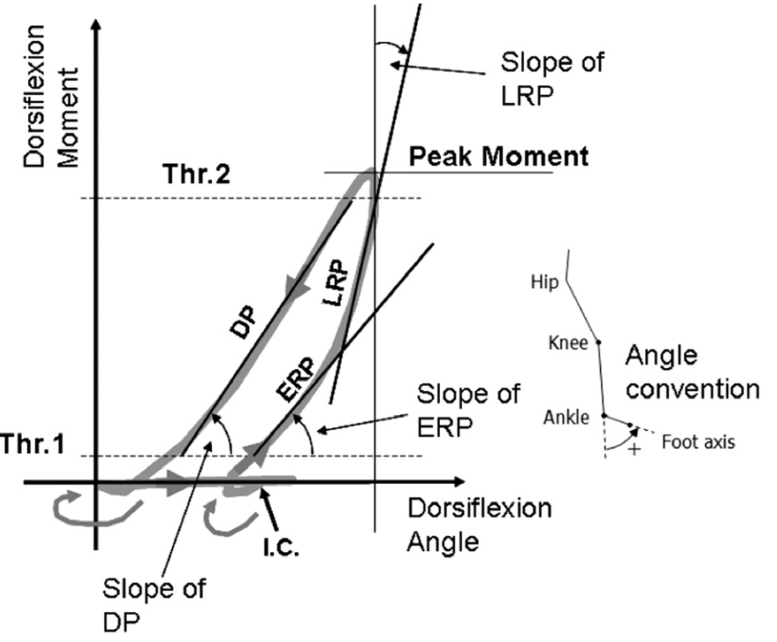
\includegraphics[scale=0.3]{slopesphases.png}
\caption{Descriptive parameters of the moment–angle loop. Taken from Crenna and Frigo\cite{Crenna2011}}
\end{center}
\end{figure}
\end{frame}

\begin{frame}[fragile]{Specific Objectives}

\begin{alertblock}{Problem Statement} 
The recent passive prosthesis for transtibial amputees produce disorders in the dynamic parameters of the gait, owing to the absence of positive work of the limb loss.
\end{alertblock}


\begin{alertblock}{General Objective} 
To suggest an ankle-foot prosthesis being able to generate --- through a passive dynamic system --- the positive work needed for push-off after dual-flexion phase, taking advantage of the energy lost at initial contact of the gait.
\end{alertblock}

\end{frame}

\section{Specific Objectives and Deliverables}

\begin{frame}{Objective No 1}
	\begin{block}{Option A}
	Through the extraction of experimental data, we will identify the biomechanical parameters and the work-loop slope in ESR prosthesis users and able-bodied people in order to obtain the ankle quasi-stiffness in both cases and establish different dynamic patterns in both.
	\end{block}
	\begin{exampleblock}{Deliverables}
	An article relating the pathological Dynamic Joint Stiffness of the ankle-joint --- and other joints if it is possible --- compared with able-bodied subjects.
	\end{exampleblock}
\end{frame}

\begin{frame}{Real experiments}
\begin{table}
\begin{centering}
\begin{tabular}{|>{\centering}p{4mm}|>{\centering}p{2cm}|>{\centering}p{2cm}|>{\centering}p{2cm}|>{\centering}p{5mm}|>{\centering}p{2cm}|}
\hline 
No. & Amputation condition & No. of subjects. & No. of trials per patient & Total. & General Observations\tabularnewline
\hline 
\hline 
1 & Bilateral & 2 & 3 & 6 & \tabularnewline
\hline 
2 & Trans-tibial & 3 left, 3 right & 5  & 30 & \tabularnewline
\hline 
3 & Trans-Femoral & 7 left, 3 right & 5 & 50 & Different speeds and sockets\tabularnewline
\hline 
\end{tabular}
\par\end{centering}
\caption{Experimental gait analysis in Colombian amputees}

\end{table}
\end{frame}

\begin{frame}{Data Available in Literature}
\begin{table}
\begin{centering}
\begin{tabular}{|>{\centering}p{4mm}|>{\centering}p{55mm}|>{\centering}p{18mm}|>{\centering}p{12mm}|}
\hline 

No. & Title & Authors & No. of subjects \tabularnewline
\hline 
\hline 
1 & \begin{scriptsize} A multiple-task gait analysis approach: Kinematic, kinetic and EMG
reference data for healthy young and adult subjects \end{scriptsize} & Bovi et al. \cite{Bovi2011} & 40 \tabularnewline
\hline 
2 & \begin{scriptsize} An elaborate data set on human gait and the effect of mechanical perturbations. \end{scriptsize} & Moore et al. \cite{Moore2015}  & 15 \tabularnewline
\hline 
3 & \begin{scriptsize} Regression analysis of gait parameters with speed in normal children
walking at self-selected speeds. \end{scriptsize} & Stansfield et al. \cite{Stansfield2006} & 16 \tabularnewline
\hline
4 & \begin{scriptsize} Benchmark Datasets for Bilateral Lower-Limb Neuromechanical Signals
from Wearable Sensors during Unassisted Locomotion in Able-Bodied Individuals \end{scriptsize} & Hu et al. \cite{Hu2018} & 10 \tabularnewline
\hline 

\end{tabular}
\par\end{centering}
\caption{Selected Studies to be analyzed}

\end{table}
\end{frame}

\begin{frame}{Data Available in Clinical Databases}
\begin{table}
\begin{centering}
\begin{tabular}{|c|>{\raggedright}p{32mm}|>{\raggedright}p{10mm}|>|c|c|c|c|c|c|>{\raggedright}p{8mm}|}
\hline 
\multirow{2}{*}{ID} & \multirow{2}{32mm}{Name} & \multirow{2}{13mm}{No. of studies} & \multicolumn{6}{c|}{Requirement} & \multirow{2}{1cm}{{\scriptsize samples accepted}}\tabularnewline
\cline{4-9} & & & 1 & 2 & 3 & 4 & 5 & 6 & \tabularnewline
\hline 
1 & Physiobank databases \cite{Physionet} & $<$100 & X & - & - & O & O & O & 0\tabularnewline
\hline 
2 & Clinical Gait analysis \cite{clinical-database} & 13 & O & X & O & O & O & O & 1\tabularnewline
\hline 
3 & Koroibot \cite{koroibot} & 544 & O & O & - & O & O & O & 10\tabularnewline
\hline 
4 & Motion Capture HDM05 \cite{HDM05} & $<$ 50 & O & O & X & O & O & O & 0\tabularnewline
\hline 
5 & CMU Graphics Lab Motion Capture \cite{Mellon} & $<$ 50 & O & - & X & O & O & - & 0\tabularnewline
\hline 
6 & MAREA Dataset \cite{Khandelwal2017} & 2 & O & O & X & - & O & O & 1\tabularnewline
\hline 
7 & ENABL3S \cite{Hu2018} & 1 & O & O & X & O & O & O & 1\tabularnewline
\hline 
\end{tabular}
\par\end{centering}
\caption{Clinical Databases found in the web.}
\label{table:Databases}
\end{table}
\end{frame}

\begin{frame}{Example of analyzed data}
\begin{figure}[H]
\begin{centering}
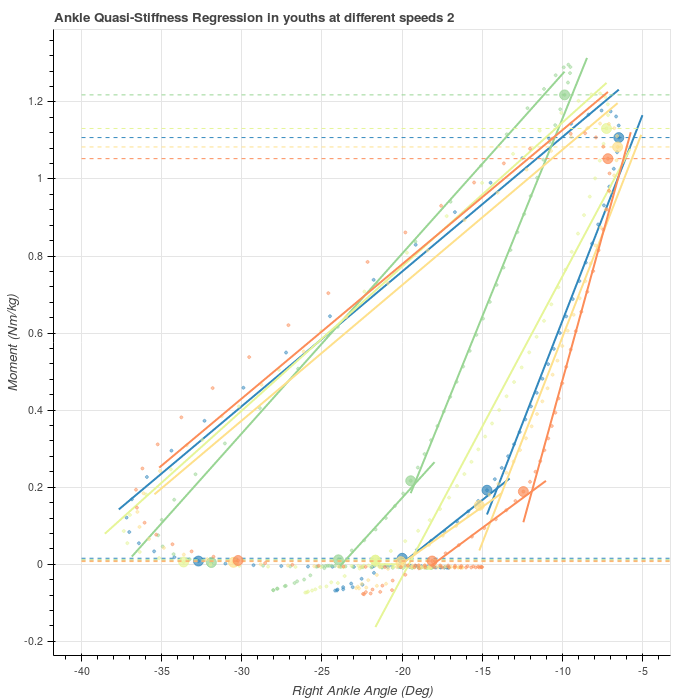
\includegraphics[scale=0.25]{quasistiffness.png}
\par\end{centering}

\caption{\label{fig:N=1} Dynamic Joint Stiffness of the ankle, being linearized according to each sub-phase of the gait}

\end{figure}
\end{frame}

\begin{frame}{Objective No. 2}
	\begin{block}{Design Optimization}
	Through the analysis of pure data found in the literature, we will attempt to give insights about the dynamic behaviour of the ankle could describe unseen aspects of different types of gait and also to identify non-linear approximations of the quasi-stiffness. 
	\end{block}
	\begin{exampleblock}{Deliverables}
	An article relating with a methodology to give an accurately prediction detecting the instances in gait or predicting relationships between different parameters of the gait (i.e. Velocity, Body length, Body mass).
	\end{exampleblock}
\end{frame}

\begin{frame}{Framework of the Biomechanical process}
\begin{figure}[H]
\begin{centering}
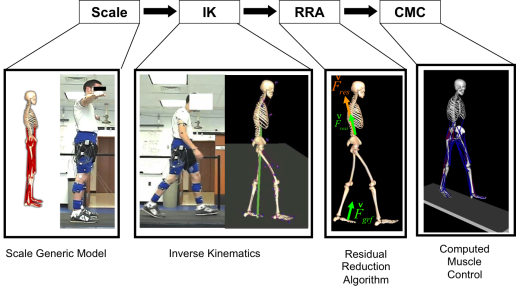
\includegraphics[scale=0.5]{opensim_process.png}
\par\end{centering}

\caption{\label{fig:N=1} Typical work-flow for generating a muscle-driven simulation after importing experimental data.}

\end{figure}
\end{frame}

\begin{frame}{Objective No. 3}
	\begin{block}{Option B}
	To get an optimal design of an ankle-foot prosthesis made mainly by composites so that the resulting macro-structure has the maximum energy returning capacity. 
	\end{block}
	\begin{exampleblock}{Deliverables}
	An article related with the framework of the design process to obtain the prosthesis and a patent probably.
	\end{exampleblock}
\end{frame}

\begin{frame}{Example of the optimization activity}
\begin{figure}[H]
\begin{centering}
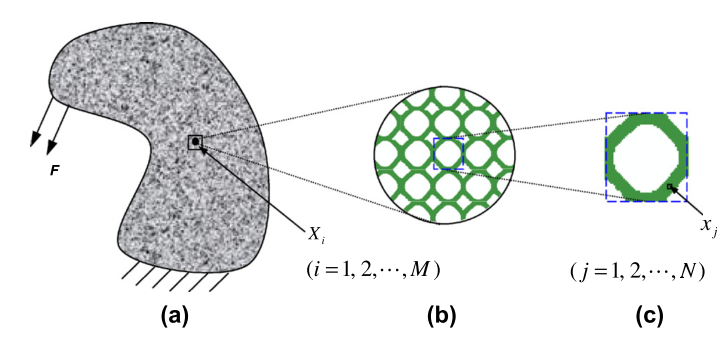
\includegraphics[scale=0.35]{optimiTopo.png}
\par\end{centering}

\caption{\label{fig:N=2} A structure composed of cellular materials or composites (a) macro-structure; (b) micro-structure; (c) a unit cell. Taken from \cite{Huang2014}}

\end{figure}
\end{frame}

\begin{frame}{Internship}
\begin{ganttchart}[
x unit=0.6cm,
y unit title=0.7cm,
y unit chart=0.8cm,
vgrid,
time slot format=isodate-yearmonth,
time slot unit=month,
title/.append style={draw=none, fill=myblue},
title label font=\footnotesize\sffamily\bfseries\color{white},
title label node/.append style={below=-1.6ex},
title left shift=.05,
title right shift=-.05,
title height=1,
bar/.append style={draw=none, fill=green!75},
bar height=.6,
bar label font=\normalsize\color{black!50},
group right shift=0,
group top shift=.6,
group height=.3,
group peaks height=.2,
bar incomplete/.append style={fill=brown},
]{2018-05}{2018-12}
%\gantttitlecalendar{year}{months} \\
\gantttitle[]{2018}{8} \\                 % title 
    \gantttitle{May}{1}
    \gantttitle{Jun}{1}
    \gantttitle{Jul}{1}
    \gantttitle{Aug}{1}
    \gantttitle{Sep}{1}
    \gantttitle{Oct}{1}
    \gantttitle{Nov}{1}
    \gantttitle{Dic}{1}\\
\ganttset{progress label text={}, link/.style={black, -to}}
\ganttgroup{Internship at IUPUI}{2018-06}{2018-12}\\ 
\ganttbar[progress=10, name=T1A]{{\footnotesize Developing computer algorithms}.}{2018-06}{2018-08} \\
\ganttbar[progress=0, name=T1A]{\footnotesize Tailoring cellular material configurations.}{2018-07}{2018-10} \\
\ganttbar[progress=0, name=T1A]{\footnotesize Physically testing cellular material configurations.}{2018-09}{2018-12} \\
\ganttbar[progress=0, name=T1A]{\footnotesize Attending lectures on Design Optimization.}{2018-06}{2018-12} \\
\ganttbar[progress=0, name=T1A]{\footnotesize Preparing one journal paper.}{2018-06}{2018-12} \\
\ganttset{link/.style={black}}
%\ganttlink[link mid=.4]{pp}{T1A}
%\ganttlink[link mid=.159]{pp}{T2A}
\end{ganttchart}

\end{frame}
\section{Bibliography}

%\begin{verse}
\begin{scriptsize}
\bibliographystyle{plain}
\bibliography{Proposal,References}

\end{scriptsize}
\section{Questions}

\begin{frame}[standout]
  Thank you!
\end{frame}

\end{document}